% !TEX root = ../7.RETENTIONTIME.tex
\section{EXPERIMENTAL THEORIES}

\subsection{Basic concept}
In the equipment system, different fluid elements will follow different paths. Based on the defined retention time distribution function, we can evaluate the flows in the equipment, identify drawbacks when designing (such as dead zones), and find ways to overcome them.

The retention time of an element in the system is the time that the element stays in the reactor. Retention time is a probability quantity. All retention times are around the average retention time; therefore, determining the average retention time is particularly significant.

\begin{equation}
    \bar{t} = \frac{\sum t_{Vi}}{n}
\end{equation}
Where $t_{Vi}$ is the retention time of element $i$.

With the definition of retention time distribution function $F(t_V) = E(t_V)$:
\begin{equation}
    E(t) = \frac{C(t)}{\int_0^{\infty} C(t) dt}
\end{equation}

Average retention time according to volume:
\begin{equation}
    \tau = \frac{V_R}{v}
\end{equation}
Where:
\begin{itemize}
    \item $V_R$: Volume of fluid in the reactor (liters).
    \item $v$: Flowrate of the input (liters/sec).
\end{itemize}

If the indicator does not reach the ideal correlation, the above equation is not satisfied. If $\bar{t} \neq \tau$, the indicator may be absorbed into the wall or there may be dead zones.

\subsection{Methods of studying retention time}
The retention time study can be carried out according to the following methods:
\begin{enumerate}
    \item Determine the composition of components at time $t$ of leaving the equipment, determine function $F(t)$.
    \item Determine the composition of components at time $t$ of still remaining in the equipment, function $I(t)$.
    \item Determine the composition of components at time $t$ of being out of the equipment, function $E(t)$.
\end{enumerate}

To survey the performance of a real reactor, we often use the stimulus-response method (marking method).

\begin{figure}[H]
    \centering
    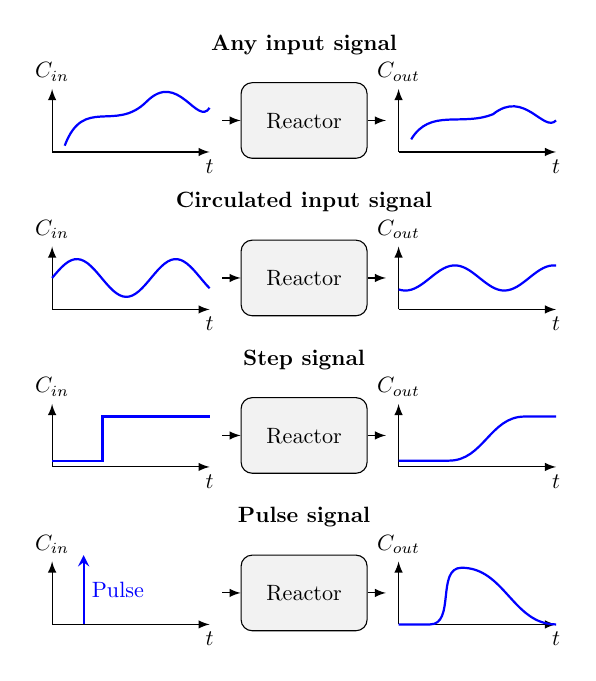
\begin{tikzpicture}[scale=0.8, every node/.style={scale=0.8}]
        % Common Styles
        \tikzset{axis/.style={-latex, thin}}
        \tikzset{signal/.style={blue, thick}}
        \tikzset{reactor/.style={draw, rectangle, minimum width=2cm, minimum height=1.2cm, fill=gray!10, rounded corners}}

        % 1. Any input signal
        \node[reactor] (R1) at (4, 0) {Reactor};
        \draw[axis] (0, -0.5) -- (0, 0.5) node[above] {$C_{in}$};
        \draw[axis] (0, -0.5) -- (2.5, -0.5) node[below] {$t$};
        \draw[signal] (0.2, -0.4) .. controls (0.5, 0.4) and (1.0, -0.2) .. (1.5, 0.3) .. controls (2.0, 0.8) and (2.3, -0.1) .. (2.5, 0.2);
        \draw[-latex] (2.7, 0) -- (R1.west);
        \draw[-latex] (R1.east) -- (5.3, 0);
        \draw[axis] (5.5, -0.5) -- (5.5, 0.5) node[above] {$C_{out}$};
        \draw[axis] (5.5, -0.5) -- (8.0, -0.5) node[below] {$t$};
        \draw[signal] (5.7, -0.3) .. controls (6.0, 0.2) and (6.5, -0.1) .. (7.0, 0.1) .. controls (7.5, 0.5) and (7.8, -0.2) .. (8.0, 0.0);
        \node at (4, 1.2) {\textbf{Any input signal}};

        % 2. Circulated input signal
        \begin{scope}[yshift=-2.5cm]
            \node[reactor] (R2) at (4, 0) {Reactor};
            \draw[axis] (0, -0.5) -- (0, 0.5) node[above] {$C_{in}$};
            \draw[axis] (0, -0.5) -- (2.5, -0.5) node[below] {$t$};
            \draw[signal, samples=50, domain=0:2.5] plot (\x, {0.3*sin(deg(\x*4))});
            \draw[-latex] (2.7, 0) -- (R2.west);
            \draw[-latex] (R2.east) -- (5.3, 0);
            \draw[axis] (5.5, -0.5) -- (5.5, 0.5) node[above] {$C_{out}$};
            \draw[axis] (5.5, -0.5) -- (8.0, -0.5) node[below] {$t$};
            \draw[signal, samples=50, domain=5.5:8.0] plot (\x, {0.2*sin(deg((\x-6)*4))});
            \node at (4, 1.2) {\textbf{Circulated input signal}};
        \end{scope}

        % 3. Step signal
        \begin{scope}[yshift=-5.0cm]
            \node[reactor] (R3) at (4, 0) {Reactor};
            \draw[axis] (0, -0.5) -- (0, 0.5) node[above] {$C_{in}$};
            \draw[axis] (0, -0.5) -- (2.5, -0.5) node[below] {$t$};
            \draw[signal] (0, -0.4) -- (0.8, -0.4) -- (0.8, 0.3) -- (2.5, 0.3);
            \draw[-latex] (2.7, 0) -- (R3.west);
            \draw[-latex] (R3.east) -- (5.3, 0);
            \draw[axis] (5.5, -0.5) -- (5.5, 0.5) node[above] {$C_{out}$};
            \draw[axis] (5.5, -0.5) -- (8.0, -0.5) node[below] {$t$};
            \draw[signal] (5.5, -0.4) -- (6.3, -0.4) node[coordinate] (start) {} to[out=0, in=180] (7.5, 0.3) -- (8.0, 0.3);
            \node at (4, 1.2) {\textbf{Step signal}};
        \end{scope}

        % 4. Pulse signal
        \begin{scope}[yshift=-7.5cm]
            \node[reactor] (R4) at (4, 0) {Reactor};
            \draw[axis] (0, -0.5) -- (0, 0.5) node[above] {$C_{in}$};
            \draw[axis] (0, -0.5) -- (2.5, -0.5) node[below] {$t$};
            \draw[signal, -stealth] (0.5, -0.5) -- (0.5, 0.6) node[midway, right] {Pulse};
            \draw[-latex] (2.7, 0) -- (R4.west);
            \draw[-latex] (R4.east) -- (5.3, 0);
            \draw[axis] (5.5, -0.5) -- (5.5, 0.5) node[above] {$C_{out}$};
            \draw[axis] (5.5, -0.5) -- (8.0, -0.5) node[below] {$t$};
            \draw[signal] (5.5, -0.5) -- (6.0, -0.5) to[out=0, in=180] (6.5, 0.4) to[out=0, in=180] (8.0, -0.5);
            \node at (4, 1.2) {\textbf{Pulse signal}};
        \end{scope}
    \end{tikzpicture}
    \caption{Frequently-used stimulus-response signals}
    \label{fig:signals}
\end{figure}

In this experiment, we use the pulse signal (Dirac delta function).

\subsection{Retention time distribution function of CSTRs model}
The general form of the distribution function for $n$ reactors in series:
\begin{equation}
    E(\theta) = \frac{n(n\theta)^{n-1}}{(n-1)!} e^{-n\theta}
\end{equation}
When $n=1$, we have an ideal CSTR model. When $n=\infty$, we have an ideal plug flow model.

Dimensionless compact time:
\begin{equation}
    \theta = \frac{t}{\tau}
\end{equation}

\begin{figure}[H]
    \centering
    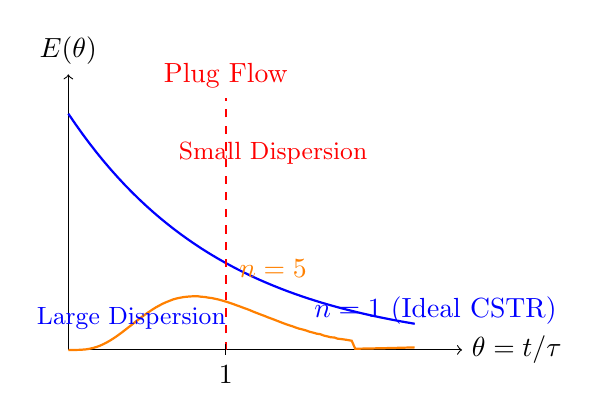
\begin{tikzpicture}[x=2cm, y=1cm]
        % Axes
        \draw[->] (0,0) -- (2.5,0) node[right] {$\theta = t/\tau$};
        \draw[->] (0,0) -- (0,3.5) node[above] {$E(\theta)$};

        % n=1 (Ideal CSTR): E(theta) = exp(-theta)
        \draw[blue, thick, samples=50, domain=0:2.2] plot (\x, {3*exp(-\x)});
        \node[blue, right] at (1.5, 0.5) {$n=1$ (Ideal CSTR)};

        % n=5: Peak at theta=1
        \draw[orange, thick, samples=100, domain=0:2.2] plot (\x, { (625/24)*(\x^4)*exp(-5*\x)*3.5 });
        \node[orange, above] at (1.3, 0.8) {$n=5$};

        % Plug Flow Model (n -> infinity): Vertical dashed line at theta=1
        \draw[dashed, red, thick] (1,0) -- (1,3.2) node[above] {Plug Flow};

        % Labels for dispersion
        \node[blue, font=\small] at (0.4, 0.4) {Large Dispersion};
        \node[red, font=\small] at (1.3, 2.5) {Small Dispersion};

        % Ticks
        \draw (1, 2pt) -- (1, -2pt) node[below] {1};
    \end{tikzpicture}
    \caption{The curve C (E-curve) showing the response at output flow for the pulse signal at the input flow for different tanks in series}
    \label{fig:e-curve}
\end{figure}
